\chapter{Despliegue de modelos de Machine Learning}\label{chap:deploy}

En los anteriores capítulos se ha explicado el flujo de trabajo seguido y levantado la infraestructura necesaria para ello, además de haber entrenado bastantes modelos con buenos resultados en lo que a métricas se refiere. Pero, ¿se ha resultado algún problema? La respuesta es no. Falta el paso más importante que desplegar nuestros modelos en la infraestructura destino o dispositivo destino.\\

En este capítulo se va a comentar cómo sería el despliegue de los modelos que están almacenados en \textit{mlflow} para levantar un microservicio o hacer funcionar un dispositivo de \textit{Edge Computing} usando un despliegue continuo. Me gustaría recalcar que nada de lo explicado en este Capítulo se ha llevado a práctica por falta de tiempo, pero no me podía olvidar de explicar lo más importante del \textit{workflow}.\\

\section{Despliegue en un microservicio}

Desplegar un microservicio es muy sencillo hoy en día gracias a servicios \textit{serverless} como \textit{AWS Lambda}, a herramientas de provisionamiento como \textit{Terraform} o de orquestación como \textit{Ansible} \cite{ansible} (para uasr un IaaS como podría ser \textit{AWS EC2}) o a servicios PaaS como \textit{Heroku}. En este último podemos desplegar aplicaciones contenedorizadas o no y contiene otros servicios de bases de datos \textit{SQL}, \textit{logging}, monitorización, etc. Por tanto, haré hincapié en este plataforma debido a que puede satisfacer más casos de uso de forma muy simple.\\

Para realizar el despliegue sería tan fácil como instalar la CLI de \textit{Heroku} (o usando herramientas de orquestación como \textit{Ansible} en el caso de IaaS) en el contenedor usado para ejecutar el \textit{pipeline} de Integración Continua y notificar en un \textit{stage} que se ejecuta al final si todos los anteriores han sido exitosos a \textit{Heroku} para volver a desplegar el contenedor o servicio actualizado.\\

Pero el problema es, ¿Cómo podemos obtener los modelos almacenados en \textit{mlflow}? Esto es bastante sencillo puesto que tiene una API para hacer \textit{queries} \cite{mlflowtrackingapi} y obtener todos los artefactos generados por un experimento, como se puede ver a continuación:\\

\begin{lstlisting}[language=Python, caption={Script de Python para obtener el modelo que maximiza la métrica \textit{test\_f1}}, captionpos=b, label=lst:getmodel]
import os
import sys
from mlflow.tracking import MlflowClient
from mlflow.entities import ViewType

tracking_uri = os.getenv("MLFLOW_TRACKING_URI")

if tracking_uri is None:
    sys.exit("MLFLOW_TRACKING_URI environment variable not defined.")

# Conexion al servidor mlflow
client = MlflowClient(tracking_uri)

# Obtener todos los experimentos
experiments = client.list_experiments()
experiments_ids = []

# Obtener todos los IDs de los experimentos
for experiment in experiments:
    experiments_ids.append(experiment.experiment_id)

# Obtener la run que maximiza la metrica test_f1
best_run = client.search_runs(
    experiments_ids,
    run_view_type=ViewType.ACTIVE_ONLY,
    order_by=["metrics.test_f1 DESC"],
    max_results=1,
)

if len(best_run) == 0:
    sys.exit("No runs found or invalid MLFLOW_TRACKING_URI.")

# Descargar el modelo almacenado en S3
best_run = best_run[0]
client.download_artifacts(
    best_run.info.run_id, path="model.pth", dst_path="artifacts"
)
\end{lstlisting}

El script anterior se encarga de recuperar el modelo que maximice la métrica \textit{test\_f1}, esto nos puede ser últil de cada a desplegarlo (incluso se podría implementar como una tarea de \textit{invoke}). Para ejecutar ese script harían falta tres variables de entorno:

\begin{itemize}
    \item \textbf{MLFLOW\_TRACKING\_URI.} Dirección de nuestro servidor de \textit{mlflow}.
    \item \textbf{AWS\_ACCESS\_KEY\_ID.} Si los modelos se guardan en \textit{AWS S3}, esta variable de entorno es necesaria para poder acceder al \textit{bucket}.
    \item \textbf{AWS\_SECRET\_ACCESS\_KEY.} Si los modelos se guardan en \textit{AWS S3}, esta variable de entorno es necesaria para poder acceder al \textit{bucket} al igual que la anterior.
\end{itemize}

\begin{lstlisting}[language=docker, caption={Dockerfile para desplegar nuestro microservicio en Heroku o en cualquier máquina}, captionpos=b]
FROM python:3.8-slim AS base

RUN groupadd python \
    && useradd -r --home-dir /home/python --shell /bin/bash -g python python \
    && mkdir /home/python \
    && chown -R python:python /home/python

USER python

ENV PATH=${PATH}:/home/python/.local/bin

WORKDIR /home/python

RUN pip install poetry

# Copiamos los ficheros importantes para el despliegue
COPY poetry.lock pyproject.toml tasks.py app/ src/ ./

# Instalamos dependencias
RUN poetry export -f requirements.txt --without-hashes | pip install -r /dev/stdin

ENTRYPOINT invoke get_model && invoke start

\end{lstlisting}

En el \path{Dockerfile} anterior se definen las órdenes necesarias para poner en producción el microservicio (siguiendo las buenas prácticas mencionadas en la Subsección \ref{subsec:dockerpractices}). Al ejecutar el contenedor creado, se llama a la \textit{task} denominada \textit{get\_model} (hace lo mismo que el script contenido en el Listing \ref{lst:getmodel}) y luego a \textit{start} (inicia el microservicio que carga el modelo para poder funcionar). Es importante definir también las variables de entorno en la máquina donde se realice el despliegue\footnote{Con \textit{Terraform} se puede editar el fichero \path{.bashrc} para establecerlas en tiempo de aprovisionamiento y en \textit{Heroku} se puede hacer fácilmente desde la interfaz \textit{web} o desde la CLI}.\\

Por último, nos queda definir el despliegue en nuestra plataforma de CI/CD. En esta ocasión, tal y como señalé en la Subsección \ref{subsec:cicdplatforms}, estoy usando \textit{Jenkins} pero puede ser cualquier otra. Para configurar el despliegue continuo, bastaría con añadir un \textit{stage} o un paso al final de todo y que se ejecute si los demás (\textit{tests} y \textit{linters}) han sido exitosos. En mi caso (ver Figura \ref{fig:jenkinspipeline}) añadiría el \textit{stage} de despliegue después del \textit{stage} paralelo que ejecuta los \textit{linters} y los \textit{tests}.\\

\begin{figure}[H]
  \centering
  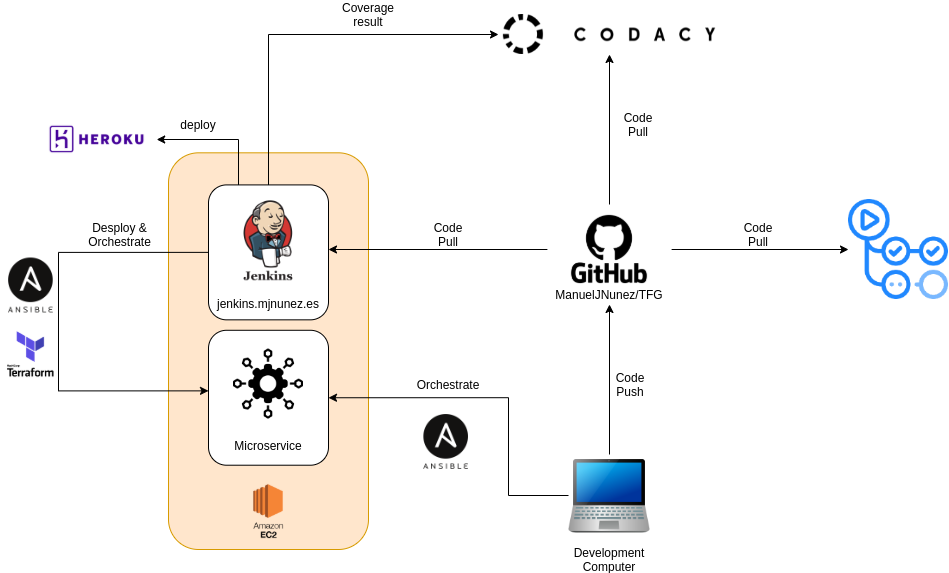
\includegraphics[width=1.\linewidth]{imagenes/07_Despliegue/TFGdiagrams-CICD.png} 
  \caption{Diagrama de cómo sería la infraestructura de \textit{testing} y de despliegue (usando \textit{Heroku} o \textit{AWS EC2}).}
  \label{fig:cicd}
\end{figure}

En la Figura \ref{fig:cicd} se muestran dos herramientas bastante importantes anteriormente nombradas, \textit{Ansible} y \textit{Terraform}. \textit{Ansible} no serviría por ejemplo para orquestar nuestra máquina o máquinas y cada vez que se producen cambios actualizar el código desplegado y volver a arrancar la aplicación. \textit{Terraform} nos valdría para controlar la infraestructura de nuestra aplicación desplegada. La infraestructura puede ser además orquestada desde la máquina de desarrollo.\\

En esta sección se ha puesto de ejemplo \textit{AWS EC2} pero se puede usar cualquier otro servicio de IaaS como \textit{GCP Compute Engine} y también se ha hablado de \textit{Heroku} pero se puede usar cualquier otro servicio de PaaS como el de \textit{Digital Ocean}. El único límite es la imaginación del desarrollador.\\

\begin{figure}[H]
  \centering
  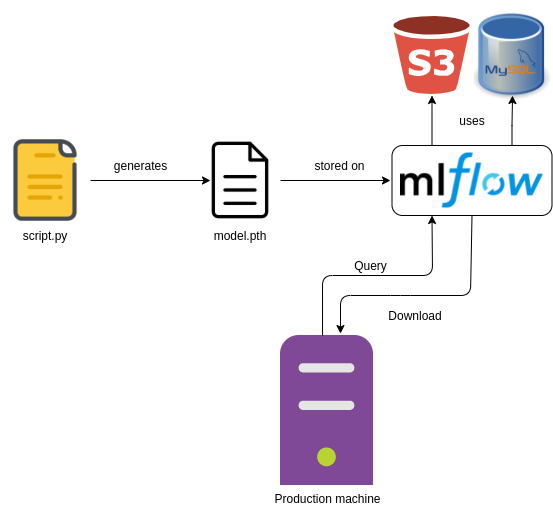
\includegraphics[width=.8\linewidth]{imagenes/07_Despliegue/ModelLifecycle.png} 
  \caption{Ciclo de vida de los modelos entrenados.}
  \label{fig:modellifecycle}
\end{figure}

En la anterior Figura \ref{fig:modellifecycle} se puede observar el ciclo de vida de un modelo desde que se genera, se serializa en un fichero que es almacenado a través de \textit{mlflow} en \textit{S3} y sus métricas e hiperparámetros son almacenados en la base de datos. La máquina en la que se mandan los modelos a producción realiza \textit{queries} (usando por ejemplo el script del Listing \ref{lst:getmodel}) para descargar el modelo que maximice la métrica objetivo.

\section{Despliegue en el contexto del \textit{Edge Computing}}

En este contexto, el diseño más habitual es el del \textit{publisher}/\textit{subscriber}. Es decir, tenemos dispositivos empotrados con sensores que publican datos y un computador central (o varios) que se subscribe a ellos a través de una red. Para la implementación de este sistema podemos usar librerías como \textit{ZeroMQ}. También podemos contar con \textit{RTI Connector} \cite{rticonnector} (una versión simple de \textit{RTI Connext DDS} para \textit{Python} y \textit{JavaScript}) que al igual que ZeroMQ no necesita de ningún \textit{broker} y podrían permitir que el diseño del sistema sea más escalable en comparación con \textit{MQTT}.\\

Como se puede ver a simple vista, este tipo de sistemas es más complejo que uno de microservicios, pues tenemos más de un dispositivo con distintas responsabilidades (unos publican por ejemplo la temperatura, otros el estado de algún objeto, otros leen los datos para procesarlos, etc). Otra dificultad que podría haber en estos dispositivos es que no tienen por qué estar 24h activos.\\

Este sería el tipo de despliegue más interesante en el contexto del problema que se pretende resolver con el conjunto de datos con el que he sido provisto (ver Sección \ref{sec:problemdesc}). Generalmente, interesa que una red de sensores sea escalable, por lo que sería interesante buscar una solución escalable que nos permita añadir nuevos nodos sin problema.\\

En este escenario, una solución basada en orquestación de contenedores (como \textit{Kubernetes} \cite{kubernetes} o \textit{Nomad} \cite{nomad}) o de orquestación de sistemas (usando \textit{Ansible} por ejemplo) sería totalmente obligatoria para controlar todo el sistema y su funcionamiento. Y no quedaría ahí, también sería esencial monitorizar todos los sistemas (se puede usar un \textit{software} como por ejemplo \textit{Grafana} \cite{grafana}, muy popular por su interfaz o \textit{Zabbix} \cite{zabbix}) y por supuesto, recoger los logs de las aplicaciones para poder ver el estado de las aplicaciones desplegadas (para ello existen herramientas online como por ejemplo \textit{logdna} \cite{logdna} o \textit{Papertrail} \cite{papertrail}). Estas herramientas no solo son útiles en el contexto de \textit{Edge Computing}, también sería interesante su uso en el despliegue de un microservicio.\\

Para monitorizar este tipo de sistemas, se puede hacer a través de la creación de un \textit{topic} denominado \textit{health} (para el caso de \textit{RTI Connector} o un tipo de mensaje especial para el caso de \textit{ZeroMQ}) a través del cual la aplicación de monitorización pregunta a todos los nodos si están funcionando correctamente. Si alguno no está funcionando no respondería y la aplicación de monitorización avisaría del estado. En el contexto de un microservicio, esto se haría mediante el uso de un \textit{health endpoint} (que devuelve 200 si todo ha ido bien). Mediante el uso de los sistemas de \textit{logging} distribuido anteriormente nombrado podemos además acceder a información sobre los mensajes de información, avisos o excepciones de las aplicaciones. Por último, recalcar que también sería necesaria la monitorización del uso de CPU, memoria, red, etc para evitar posibles saturaciones del sistema.
